\documentclass[text05.tex]{subfiles}
\begin{document}
\subsubsection{\ruby{傾斜}{けい|しゃ}センサー}\label{tilt}
\begin{table}[H]
  \begin{widerrows}
    \begin{tabular}{|p{\colF}|p{\colG}|}	\hline
    \ruby{名称}{めい|しょう} & \ruby{傾斜}{けい|しゃ}センサー（けいしゃせんさー）\\ \hline
    \ruby{接続箇所}{せつ|ぞく|か|しょ} & デジタルコネクタ (3pin)\\ \hline
    \ruby{機能概要}{き|のう|がい|よう} & 中のボールの転がりで、\ruby{傾}{かたむ}きを\ruby{検知}{けん|ち}する\\ \hline
    \end{tabular}
  \end{widerrows} 
\end{table}

\begin{table}[H]
  \begin{widerrows}
    \begin{tabular}{|p{\colF}|p{\colG}|}	\hline
    サンプルコードの場所 & 05/digin.hsp\\ \hline
    raspiへの入力 & センサーの向きによって中のボールが\ruby{端子}{たん|し}に\ruby{触}{ふ}れると1、\ruby{触}{ふ}れないと0の\ruby{値}{あたい}を入力します。\\ \hline
    raspiへの入力方法 & val = gpioin(GPIO番号)\\ \hline
    raspiからの出力 & なし\\ \hline
    raspiからの出力方法 & なし\\ \hline
    \end{tabular}
  \end{widerrows} 
\end{table}

\begin{figure}[H]
  \begin{widerrows}
    \begin{tabular}{|p{\colF}|p{\colG}|} \hline
    使い道 & ストーブの安全\ruby{装置}{そう|ち}\\ \hline
    \ruby{注意事項}{ちゅう|い|じ|こう} & なし\\ \hline
    \ruby{補足}{ほ|そく} & 黒い箱のなかにボールが入っていて、ボールが転がり\ruby{端子}{たん|し}に\ruby{触}{ふ}れるとONになります。\ruby{傾}{かたむ}いていないときはOFFになります。
    \par
    \begin{minipage}[t]{\linewidth}
      \smallskip
        \centering
        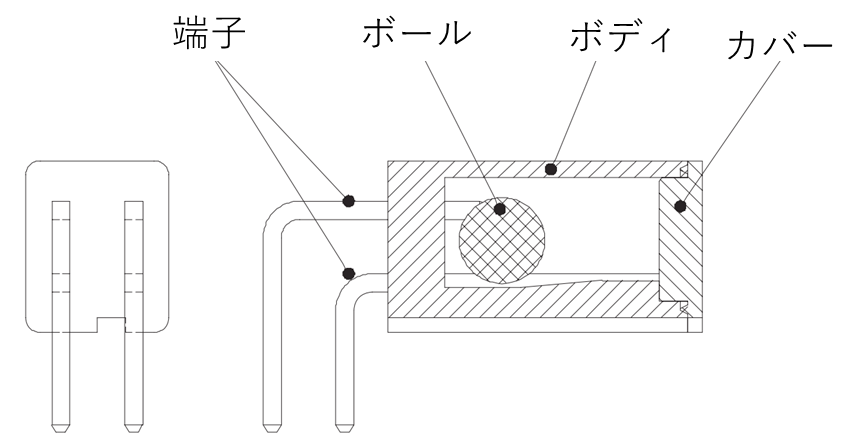
\includegraphics[width=0.7\linewidth]{../../asset/image/text05-img046.png}
        \caption{\ruby{傾斜}{けい|しゃ}センサーの内部}
        \smallskip
      \end{minipage}
    \\ \hline
    \end{tabular}
  \end{widerrows} 
\end{figure}

\begin{figure}[H]
  \begin{widerrows}
    \begin{tabular}{|p{\colH}|p{\colI}|p{\colH}|p{\colI}|} \hline
    外観 & 
    \begin{minipage}[t]{\linewidth}
      \smallskip
        \centering
        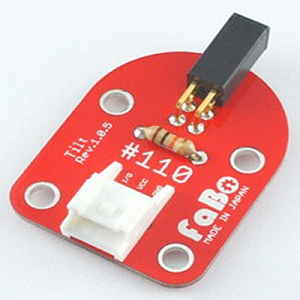
\includegraphics[width=0.5\linewidth]{../../asset/image/text05-img018.png}
        \caption{\ruby{傾斜}{けい|しゃ}センサー}
        \smallskip
      \end{minipage} &
      回路記号 & 
      \begin{minipage}[t]{\linewidth}
      \smallskip
        \centering
        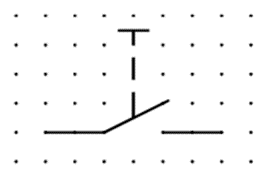
\includegraphics[width=0.5\linewidth]{../../asset/image/text05-img047.png}
        \caption{\ruby{傾斜}{けい|しゃ}センサーの回路図}
        \smallskip
      \end{minipage}\\ \hline
    \end{tabular}
  \end{widerrows} 
\end{figure}\end{document}
